\chapter{Accretion Disc Winds}
\label{sec:winds}

\epigraph{``A view of space, with an elephant obstructing it"}
{{\sl Mike Vennart, Silent/Transparent}}


%%%%WINDS 
%%% COULD MAKE THIS A NEW CHAPTER
\section{Observational Evidence}

The observational evidence for mass-loaded outflows or winds is 
widespread across the entire astrophysical mass range and most of
the electromagnetic spectrum. Before detailing the more compelling aspects
of this evidence, it is pertinent to briefly discuss the `smoking gun'
used to unambiguously detect winds -- the presence of blue shifted BALs
or `P-Cygni' profiles in an objects spectrum. 

\begin{figure}
\centering
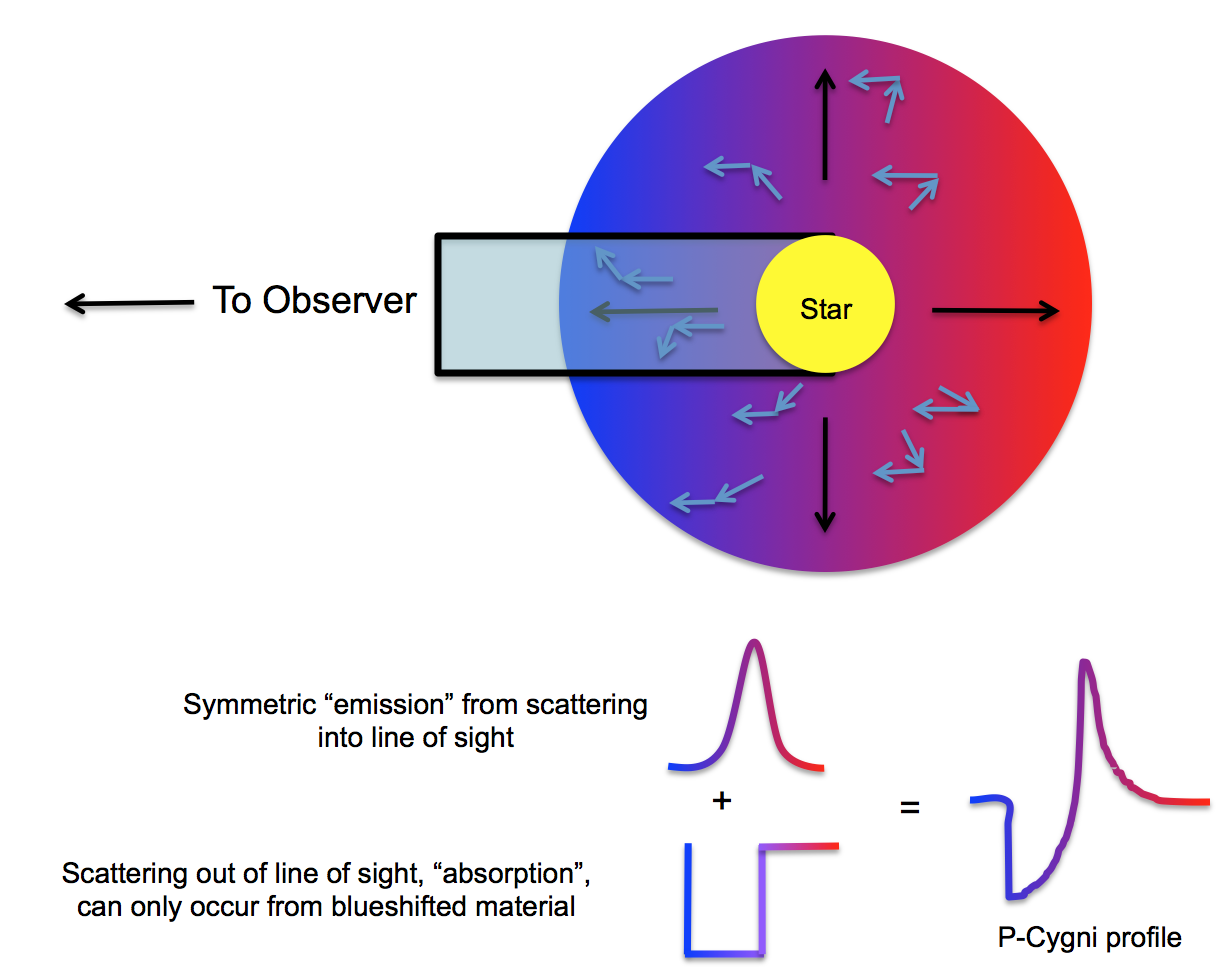
\includegraphics[width=1.0\textwidth]{figures/02-outflows/pcyg.png}
\caption
{
Diagram showing how an expanding envelope or wind with significant line
opacity around a continuum source leads to the formation of P-Cygni profiles.
The black arrows denote the outflow direction and the blue arrows typical
scattering interactions.
} 
\label{fig:pcyg}
\end{figure}

Figure~\ref{fig:pcyg} shows how a spherical outflow of significant opacity will 
cause these characteristic line profile shapes to form, 
as scattering out of the line of sight 
causes a dip in the blue wing of the line, while scattering into the 
line of sight from other portions of the outflow causes an increase in flux
in the red wing of the line. The situation is much more complex in most
astrophysical situations; for example, the geometry is rarely spherically 
symmetric, and the line is rarely a pure scattering case. Indeed, the potential 
for complicated radiative transfer effects and variety in line formation mechanisms
is one of the reasons why 3D Monte Carlo radiative transfer simulations are necessary
to effectively model disc winds (see section 3).



\subsection{Cataclysmic Variables}

It has been known for a long time that winds emanating from the
accretion disc are important in shaping the ultraviolet (UV) spectra
of high-state CVs \citep{heap1978, greensteinoke1982}. 
The most spectacular evidence for such
outflows are the P-Cygni-like profiles seen in UV resonance lines such as
\civfull\ \citep[][see figure~\ref{fig:cordova}]{cordova1982}). 
Considerable effort has been spent over the
years on understanding and modelling these UV features 
\citep[e.g.][]{drewverbunt1985,maucheraymond1987,SV93,KWD95,
kd1997,knigge1997,LK02,noebauer,puebla2011}. 
The basic picture emerging from these efforts is
of a slowly accelerating, moderately collimated bipolar
outflow that carries away $\simeq 1\% - 10\%$ of the accreting
material. State-of-the-art simulations of line formation in this type
of disc wind can produce UV line profiles that are remarkably similar
to observations, as shown in figure~\ref{fig:zcam_lk02}.

\begin{figure}
\centering
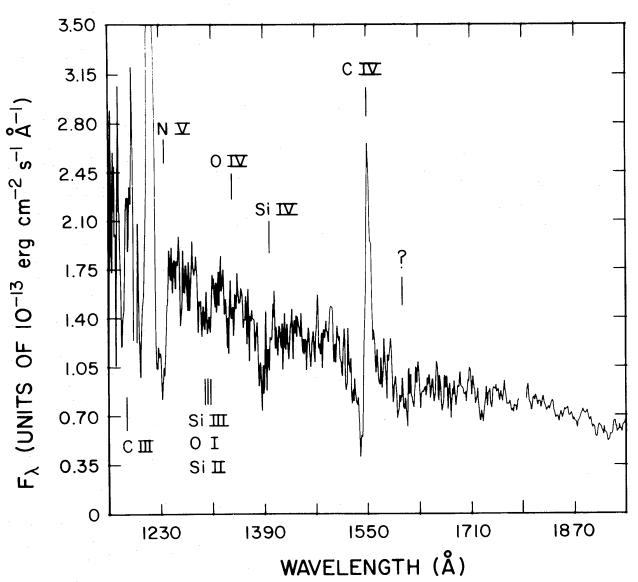
\includegraphics[width=0.8\textwidth]{figures/02-outflows/cordova_mason.png}
\caption
{
{\sl Credit: Cordova \& Mason 1982}. 
UV spectrum of the DN TW Vir during outburst. The P-Cygni profiles
can be seen clearly, demonstrating that a strong, fast outflow is present
in the system. 
} 
\label{fig:cordova}
\end{figure}

\begin{figure}
\centering
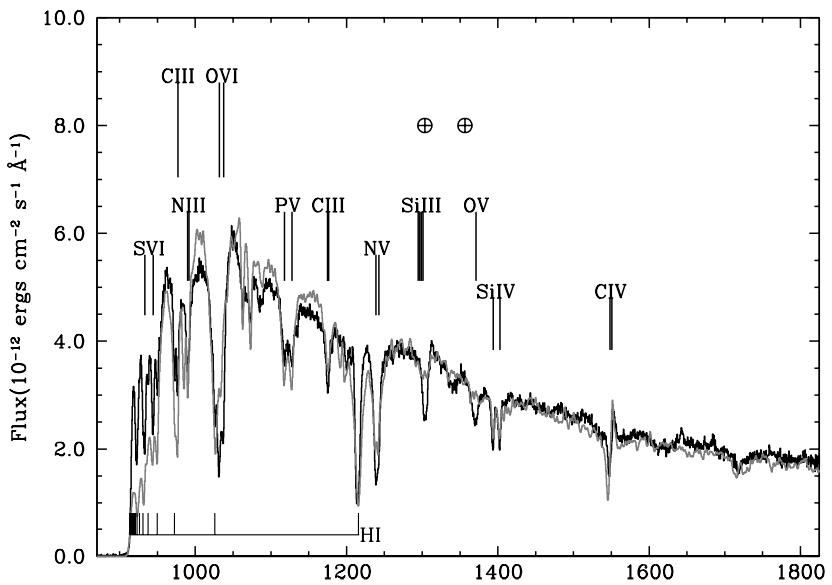
\includegraphics[width=0.8\textwidth]{figures/02-outflows/zcam_lk02.png}
\caption
{
{\sl Credit: Long \& Knigge 2002}. 
UV spectrum of Z Cam, compared to a synthetic spectrum from MCRT simulations.
} 
\label{fig:zcam_lk02}
\end{figure}

Much less is known about the effect of these outflows on the optical
spectra of high-state CVs. Direct evidence of wind-formed lines comes from
isolated observations of P-Cygni-like line profiles in
\ha\ and He \textsc{i} $\lambda5876$, \citep{patterson1996, RN98, kafka2004}. 
However, the effect on
the {\em emission} aspects of the optical spectrum is not well known.
\cite{MC96, MC97} have shown that the presence of disc winds may
offer a natural explanation for the single-peaked optical emission lines in
high-state CVs, since they can strongly affect the radiative transfer
of line photons (see figure~??). Stronger support for a significant wind contribution to the
optical emission lines comes from observations of eclipsing
systems. There, the single-peaked lines are often only weakly
eclipsed, and a significant fraction of the line flux remains visible
even near mid-eclipse \citep[e.g.][]{baptista2000,groot2004}. 
This points to line formation in a spatially
extended region, such as a disc wind (see section~\ref{novalikes}).
It is also possible that a wind may affect the continuum emission of CVs,
as described in section~??. The effect of an accretion disc wind
on the optical line and continuum emission of CVs is addressed directly,
via radiative transfer modelling, in chapter 4.

% These spectra are typically characterized
% by H and He emission lines superposed on a blue continuum. In many
% cases, and particularly in the SW~Sex subclass of NLs
% \citep{HSK86,DR95}, these lines are single-peaked. This is contrary to
% theoretical expectations for lines formed in accretion discs, which
% are predicted to be double-peaked \citep{smak1981, hornemarsh1986}. 
% {\em Low-state} CVs (dwarf novae in quiescence) do, in fact,
% exhibit such double-peaked lines \citep{marshhorne1990}. 

% Could disc winds also have an impact on the UV/optical {\em continuum}
% of high-state CVs? This continuum is usually thought to be dominated
% by the accretion disc and modelled by splitting the disc into
% a set of concentric, optically thick, non-interacting annuli following
% the standard $T_{eff}(R) \propto R^{-3/4}$ radial temperature
% distribution \citep{shakurasunyaev1973}. In such
% models, each annulus is taken to emit either as a blackbody or,
% perhaps more realistically, as a stellar/disc atmosphere model
% \citep{Schwarzenberg-Czerny1977,wade1984,wade1988}.
% In the latter case, the local surface gravity, $\log{g}(R)$, is
% assumed to be set solely by the accreting WD, since self-gravity is
% negligible in CV discs.

\subsection{X-ray Binaries}
\label{sec:xrb_winds}

Like CVs, evidence for fast outflows in LMXBs is not constrained to 
a single waveband. UV absorption in outflows was detected when
\cite{ioannau2003} observed \civfull\ P-Cygni profiles with blueshifts 
of $\sim1500$km~s$^{-1}$. Shortly after, a series of papers found 
highly ionized Fe absorption with similar blueshifts and FWHM of around 
$1500$km~s$^-1$ (REFs). These absorption features tended to be detected
in high-inclination, `dipping' LMXBs, and this was confirmed in more sources
by \cite{ponti2012}, who proposed an equatorial geometry based on this (see 
figure~\ref{fig:ponti_cartoon}). 
The same study demonstrated (figure~\ref{fig:ponti_hid}) that
the winds only appeared in the soft, 
disc dominated accretion state, on the opposite side of the HID to the
region where jets are common. This exciting result demonstrated how
important winds are to our understanding of accretion, and required that
we expand the discussion of accretion states from `disc-jet' coupling
to also include winds.

\begin{figure}
\centering
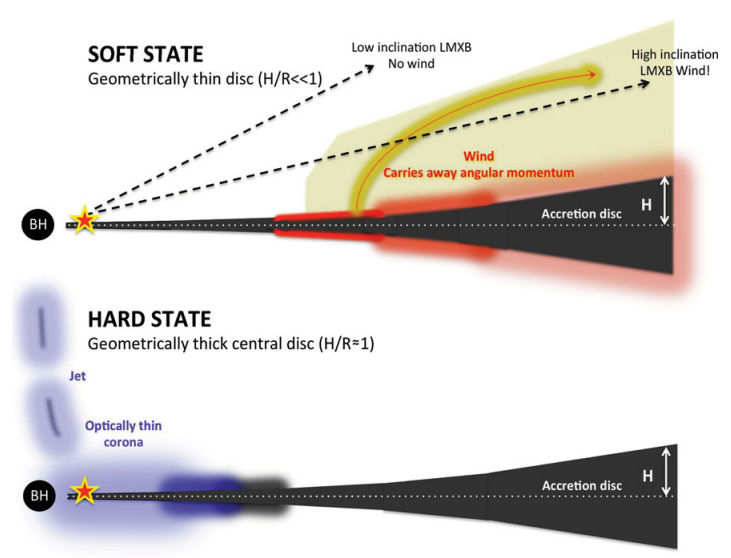
\includegraphics[width=0.8\textwidth]{figures/01-intro/ponti_wind_cartoon.png}
\caption
{
{\sl Credit: Ponti et al. 2012}. 
A cartoon illustrating the expected geometry of soft-state LMXB winds.
} 
\label{fig:ponti_cartoon}
\end{figure}


\begin{figure}
\centering
\includegraphics[width=0.8\textwidth]{figures/01-intro/ponti_hid.png}
\caption
{
{\sl Credit: Ponti et al. 2012}. 
Hardness-intensity diagram for four dipping LMXBs,
demonstrating that winds appear only in the soft state.
} 
\label{fig:ponti_hid}
\end{figure}


\subsection{AGN and Quasars}
\label{sec:agn_winds}

\subsubsection{Broad Absorption Line Quasars}

\begin{figure}
\centering
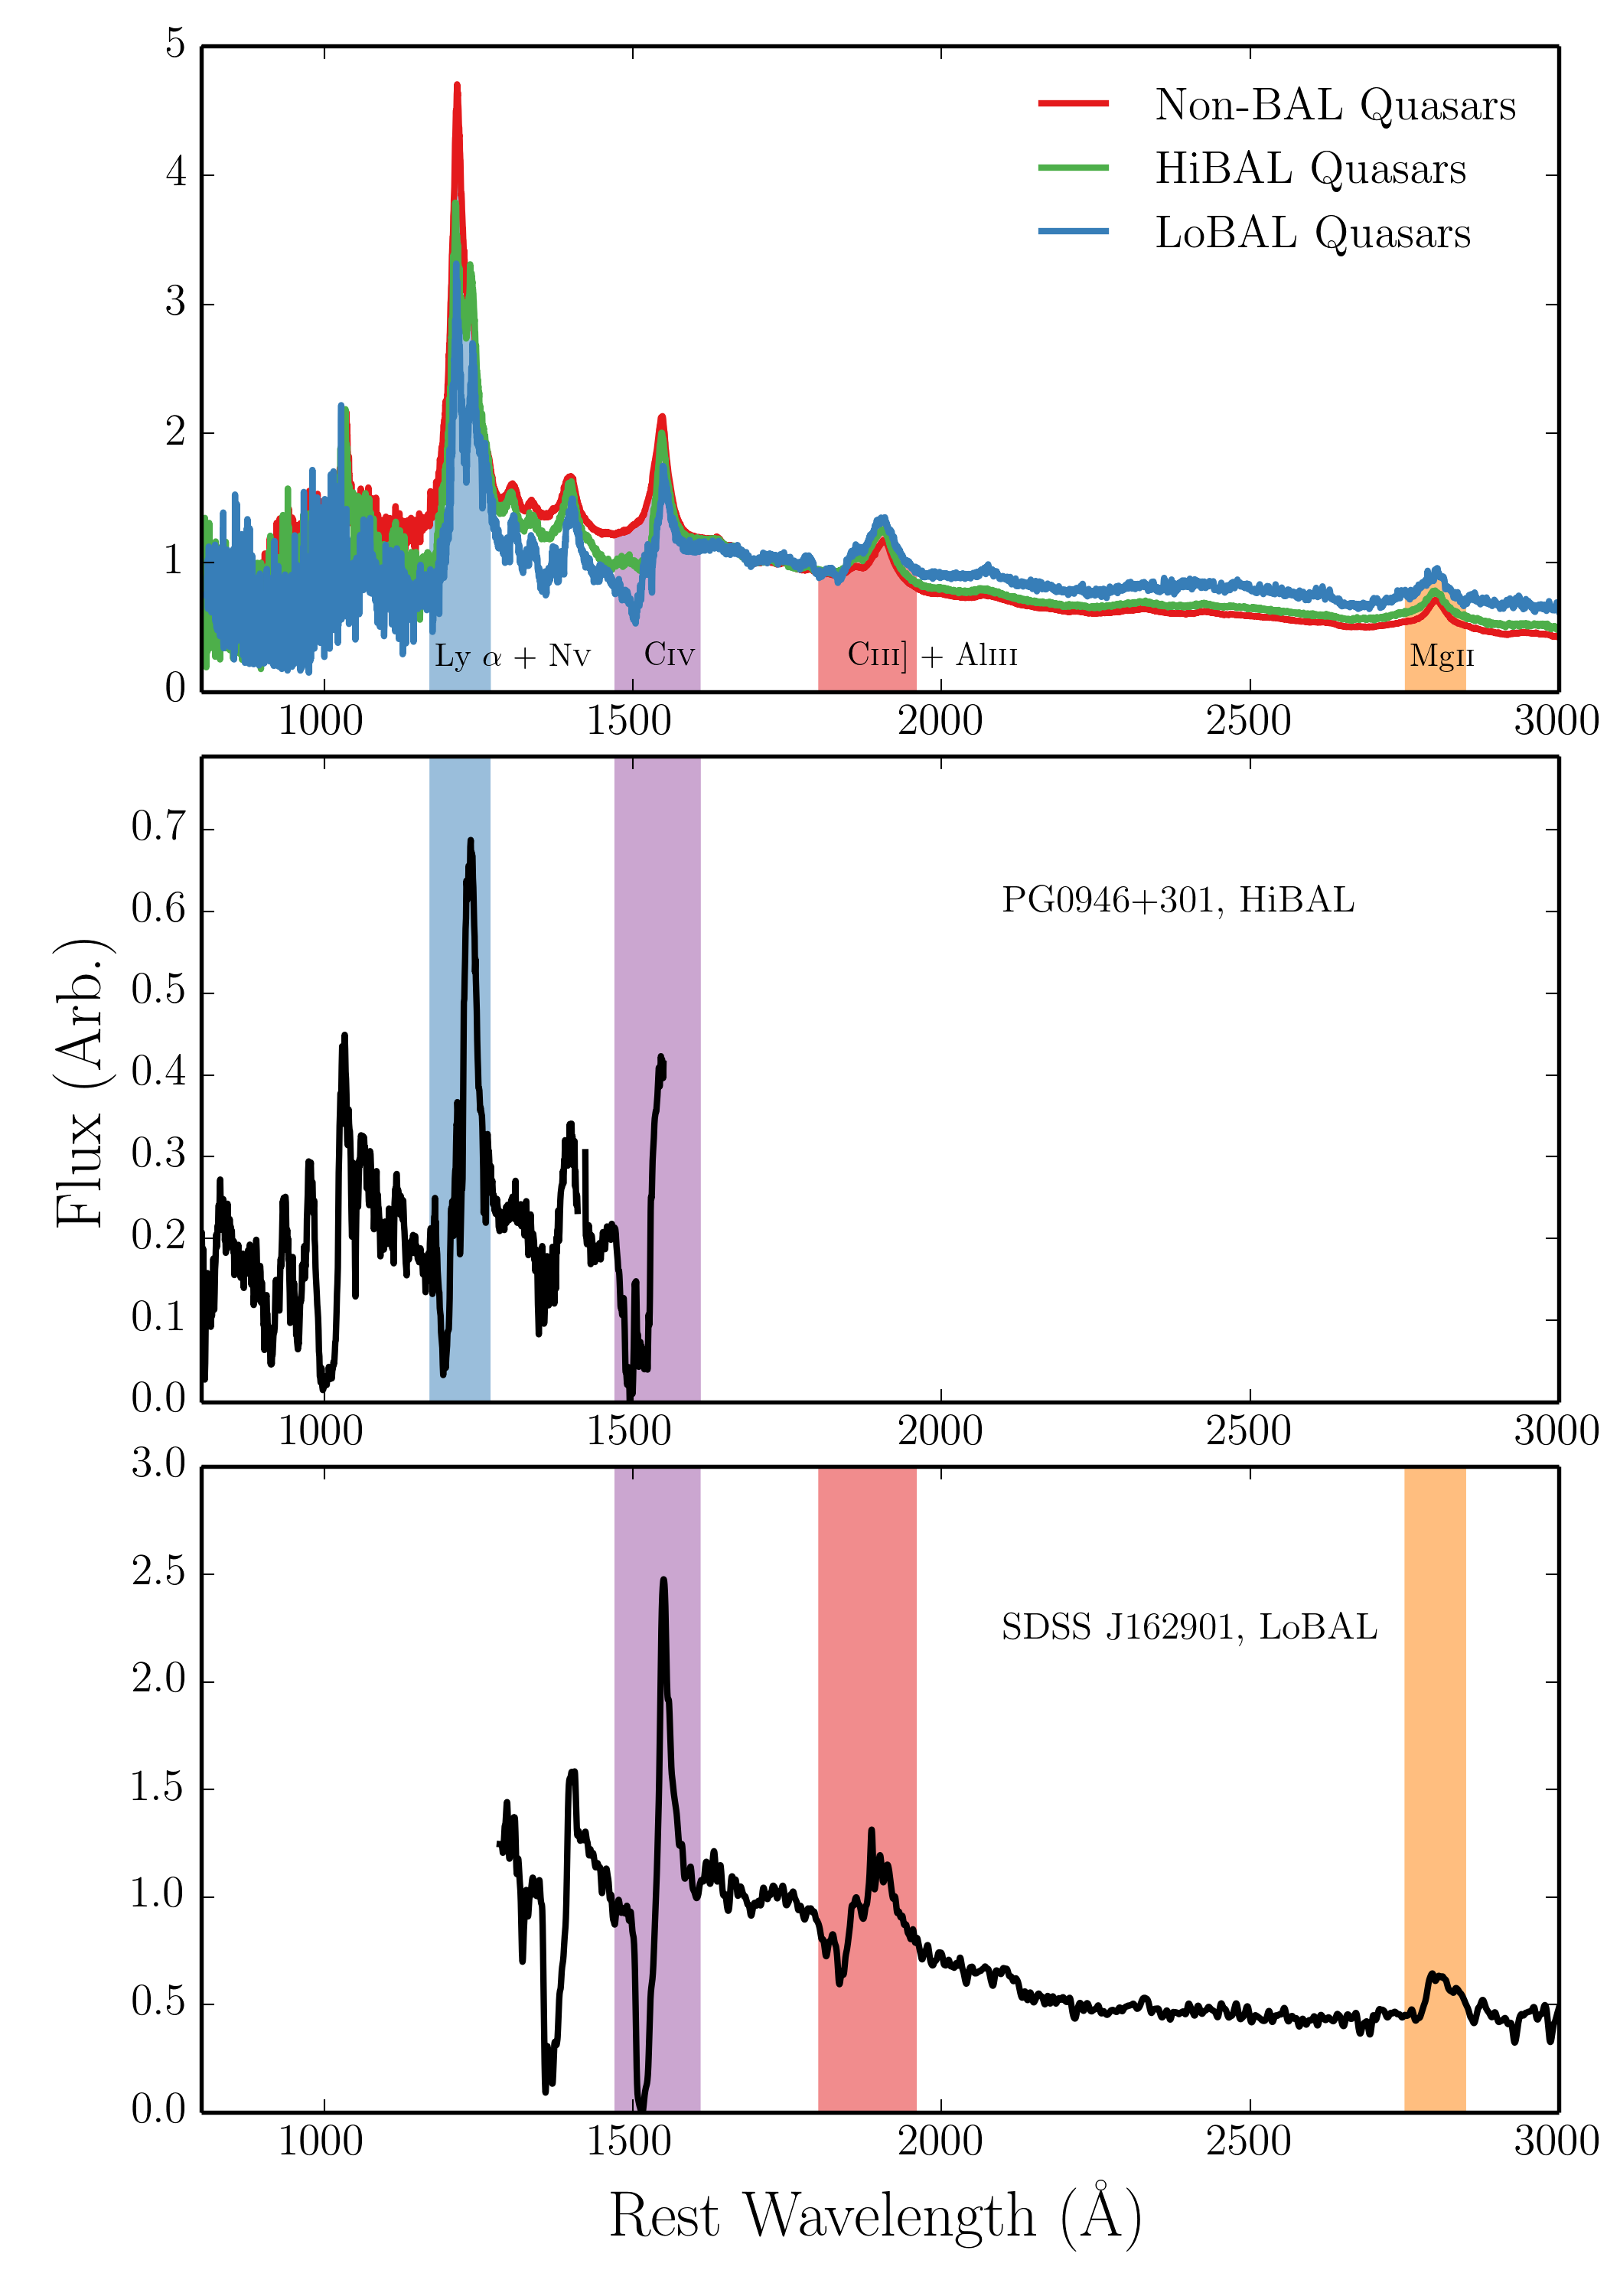
\includegraphics[width=1.0\textwidth]{figures/02-outflows/bal_spectra.png}
\caption
{
Five examples of BAL quasar spectra, from HST and SDSS.
} 
\label{fig:bals}
\end{figure}

Perhaps the clearest evidence of outflows in AGN is  
the blueshifted ($\sim 0.1~c$) broad absorption lines (BALs) in the 
ultraviolet seen in approximately $20-40\%$ of quasars
\citep{weymann1991, knigge2008, dai2008, allen2011}. Five example
spectra of BAL quasars from the HST and SDSS archives are shown in 
figure~\ref{fig:bals}. In addition to the most common High-ionization
BAL quasars (HiBALs), approximately $10\%$ of BALQSOs show absorption
in lower ionization species such as \mgii\ and \aliii\ 
\citep[LoBALs; ][]{voit1993,gibson2009}
and an even smaller subset also show absorption in Fe~\textsc{ii} and 
\textsc{iii} \citep[FeLoBALs; ][]{becker2000,hall2002}. 

The simplest explanation for the incidence of 
BAL quasars (BALQSOs) is in terms of an accretion disc wind viewed
from different angles. This principle of geometric unification
is very similar to the idea behing the UP95 and AM95 models discussed in Chapter 1.
According to this paradigm, a biconical wind rises from 
the accretion disc and the BALQSO fraction is associated with
the covering factor of the outflow. This fraction
has been estimated by various authors using different selection criteria, with
values ranging between $10$ and $40\%$ depending on corrections 
and the classification scheme used 
\citep{weymann1991, trump2006, knigge2008, dai2008, allen2011}

BAL quasars can also interpreted in an {\em evolutionary}
context, in which quasars spend a certain proportion of their life
in the `BAL phase'. Models generally put this phase near the start
of the quasar lifetime \citep{hazard1984,surdej1987,boroson1992,zubovas2013}, 
after a dust enshrowded phase but before
the main quasar period. It is perhaps more likely that {\em both} 
evolutionary and geometric effects are at work \citep{borguet2010,dai2012}.
One of the main problems with testing these two paradigms is that many of
the properties of BAL quasars fit naturally into either picture, and so
disentangling their true nature if challenging. 
The latter chapters of this thesis attempt to address this issue by testing the 
geometric unification model, or `Occam's quasar' (see Chapter 1),
and establishing how close this simple picture can get to explaining 
the BAL phenomenon.  

While the BAL fraction, $f_{BAL}$, is a very useful number and must be at least
related to the covering factor of the outflow, continuum selection
effects \citep{goodrich1997,krolikvoit1998}, 
as well as reddening \citep{allen2011}, could significantly
alter the true value of $f_{BAL}$. The degree of collimation of the BAL wind
is also not well known. Polarisation studies suggest that the 
wind is roughly equatorial \citep{goodrich1995, cohen1995}, 
as also found from hydrodynamical and radiative transfer simulations 
\citep{PSK2000,PK04, higginbottom2013},
but there is also evidence for polar BAL outflows in 
radio-loud (RL) sources \citep{zhou2006,ghoshpunsly2007}.
In addition to these uncertainties, the physical scale of the BAL
phenomenon is also disputed, and may vary from object to object.
If one assumes that the BAL region is on the same scale as 
the BLR then the radius of the absorbing material
can be estimated as $\sim 100-1000 r_G$ from reverberation mapping
and microlensing \citep[e.g., for BLRs in BALQSOs,][]{sluse2015,odowd2015}.
However, distances of  $\sim0.1$~pc ($\sim 10^4 r_G$) have been measured in at least 
some objects from atomic physics arguments and ionization models
\citep{borguet2013,chamberlain2015}.

BAL quasars display a variety of different trough shapes from object 
to object, as shown in figure~\ref{fig:bals}. The 
line profiles themselves often show complex structure 
\citep{foltz1987,ganguly2006, simonhamann2010} and can be time variable 
\citep{hall2011, capellupo2011,capellupo2012,capellupo2014, filizak2012}. 
Furthermore, there are a set of quasar absorption systems that show
BAL-like absorption troughs with much smaller velocity widths. Depending 
on their width, these are known as narrow absorption lines (NALs) or `mini-BALs'
\citep{misawa2007,misawa2008,nestor2008,hamann2012}.
While some of this behaviour can be explained once again as a viewing angle
effect \citep[e.g. ][]{ganguly2001}, the range of BAL profile shapes suggests that they 
are far from a homogenous population, and may also possess
multi-scale substructures (clumps) in their flows. Clumping
is discussed in more detail in sections~\ref{sec:stellar_winds} and 
\ref{sec:rad_winds}, as well as in Chapter 6.

Due to the connection between X-rays and photoionization / absorption, the 
X-ray properties of BAL quasars are particularly important. BALQSOs
are universally X-ray weak when compared to non-BAL quasars \citep{gibson2009}. 
The X-ray weakness of BALQSOs is often attributed to X-ray absorption 
with column densities of $N_H \sim 10^{22-24}$~cm$^{-2}$ 
\citep{gallagher1999,gallagher2002,green2001,grupe2003,stalin2011},
although there is also evidence that BALQSOs are {\em intrinsically}
X-ray weak \citep{sabra2001,clavel2006,morabito2013}.
The X-ray properties of BAL quasars are fundamentally coupled to 
the properties of the wind -- the X-ray absorption may be caused by 
the outflow which in turn has its ionization state 
determined by the X-ray radiation. Furthermore, the true X-ray 
luminosities cannot be reliably inferred until inclinations of BALQSOs are
constrained, as gravitational lensing will significantly alter the
emergent angular distribution of X-ray emission even for an intrinsically
isotropic source \citep{chen2013a, chen2013b}.

Although the X-rays in BALQSOs are weaker than in similar mass quasars,
they still possess strong ionizing power. This leads to what has become
known as the `over-ionization problem' in BALQSOs; how is the moderate 
ionization state of the BAL gas maintained in the presence of ionizing 
X-rays? A number of potential solutions have been proposed, which can be 
broadly separated into `shielding' models \citep{MCGV95,PK04} and `clumpy'
models \citep{dekool1995,hamann2013}. Some of these models are discussed
further in section~\ref{sec:wind_models} and chapter~5.

\subsubsection{Warm Absorbers}

Warm absorbers (WAs) are regions of photoionized plasma responsible for some
of the characteristic absorption features seen in the 
X-ray spectra of AGN \citep{reynolds1995}.
In particular, they produce photoelectric continuum absorption 
\citep[e.g.][]{halpern1984,cappi1996,kriss1996}
and a series of narrow absorption lines in H-like and He-like ions of 
C, N, O, Si, Ne, and Fe \citep{kaastra2000}, that appear in the soft X-rays.
A wind origin is a common hypothesis for WAs 
\citep[e.g.][]{krolikkriss2001}. Clear evidence for this 
comes from the measured blueshifts of the lines, typically on the order of 
$\sim100$km~s$^{-1}$. X-ray absorption and WAs are often
variable \citep{fabian1994,otani1996}, which may be interpreted in terms of 
changing kinematics of an accretion disc wind \citep{connolly2014}. 
There is also evidence of contemporary UV and X-ray absorption 
in NGC 5548 \citep{kaastra2014} and mini-BALS \citep{giustini2011},
and as mentioned above BALQSOs 
are often absorbed in the X-rays. This suggests that the outflow phenomenon 
across a large range of ionization states and line energies is linked. 

WAs can, in some cases, be modelled well with single component 
models \citep{kaastra2000}, but often
require multiple ionization state absorbers 
\citep[e.g.][]{kriss1996,orr1997,krolikkriss2001,connolly2014}.
If this is the case, then self-consistent ionization and radiative transfer models
should really be used to model the spectrum (see e.g. chapter 3), 
as optically thin ionization parameter estimates will not capture 
the ionization and radiation physics.
The collated observations point towards some kind of outflow with a stratified ionization
structure, with $\log \xi \sim 0-2$, and densities on the order of $10^8$~cm. 
These physical conditions or scales are not well constrained, and the connection to 
other outflows is unknown. Timing observations will help to shed light on 
the properties of the mysterious, but ubiquitous, 
AGN WAs \citep{silva2015}.

\subsubsection{Ultra-fast Outflows}

As well as acting as WAs, winds also imprint clear absorption features
in highly ionized Fe~K$\alpha$ lines in AGN such as PDS~456 
\citep{reeves2003, gofford2014,matzeu2016},
MCG-5-23-16 \citep{braito2007} and PG 1211+143 \citep{poundsreeves2009,fukumura2015}.
These features are fairly common in Seyfert galaxies \citep{tombesi2010a, gofford2013}. 
An example of such a feature is shown in 
figure~\ref{fig:nardini} with a simply spherical outflow model fit, 
from \citep{nardini2015}. The high velocities ($\sim0.1c$) inferred 
from the line blueshifts have lead to these winds becoming known as 
ultra-fast outflows, or UFOs. 

UFOs are characterised by ionization parameters of $\log \xi \sim 3-4$,
and column densities of $N_H > 10^{22}$~cm$^{-2}$. Their high mass-loss rates
and large energy budgets mean that they are natural candidates for
AGN feedback (see section~\ref{sec:agn_feedback}). Measurements of
their kinetic luminosities suggest that UFOs do have sufficient 
energy to affect their host galaxy \citep{gofford2015}, and a recent observation
showed a molecular outflow in a UFO host galaxy, possibly driven 
by the UFO itself \citep{tombesi2015}. As with WAs, many of the models
used to constrain physical parameters are simplistic, and assume 
single ionization parameters, large covering factor
and thin expanding shells of outflow.
Under these assumptions, the mass loss rate can be estimated using
\begin{equation}
\label{eq:hse}
\dot{M} \sim \Omega N_H m_p v_{out} R_{in}
\end{equation}
In reality, the absorber is probably much more complex, and full 
RT and photoionization simulations are required. In a series of papers, 
\cite{simlong2008,sim2010,sim2010_hydro} carried out such calculations,
and found reasonable verisimilitude with Fe line profiles could be achieved.
However, as with many models for AGN, a holistic, broad wavelength range
fit is still required.

\begin{figure}
\centering
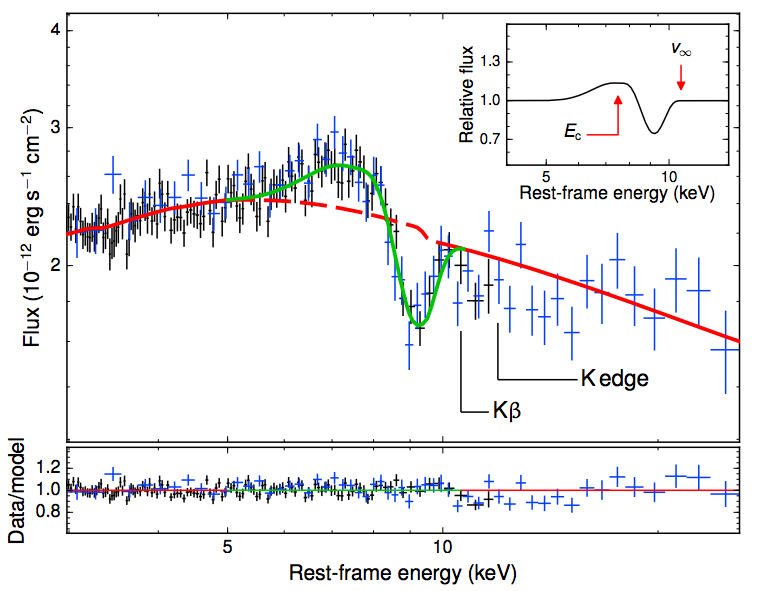
\includegraphics[width=1.0\textwidth]{figures/02-outflows/nardini_pds456.png}
\caption
{
{\sl Credit: Nardini et al. 2015}. 
X-ray spectrum of PDS 456 fitted with a P-Cygni profile from a 
spherical outflow model. {\sl XMM-Newton} data is shown in black 
with two combined {\sl NuStar} observations in blue.
} 
\label{fig:nardini}
\end{figure}


\subsection{Stellar Winds}

\label{sec:stellar_winds}

Although stellar winds are clearly not accretion disc winds,
they provide a useful, and better understood, testing ground for much
of the physics of radiatively-driven outflows. 
Wolf-Rayet stars and O-stars

\nocite{pauldrach1994}
\begin{figure}
\centering
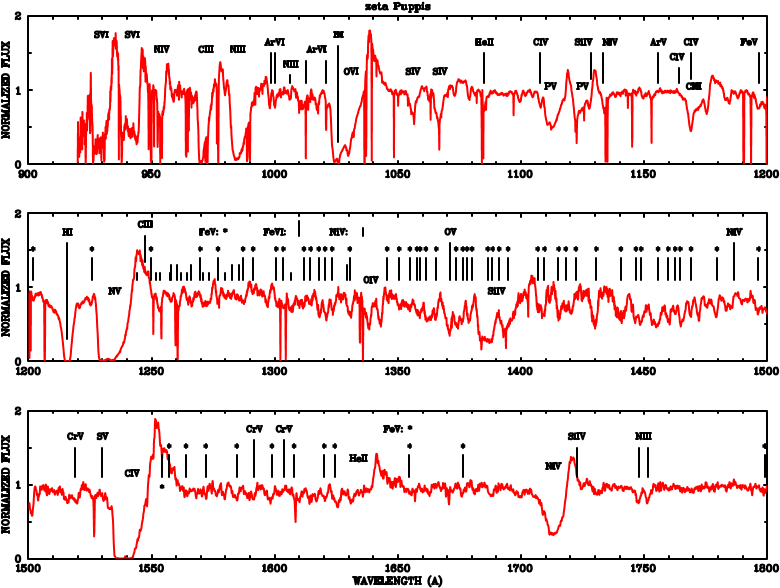
\includegraphics[width=1.0\textwidth]{figures/02-outflows/hot_star_wind.png}
\caption
{
{\sl Credit: Pauldrach et al. 1994}. 
UV spectrum of one of the brightest massive O stars, 
the O4 supergiant $\zeta$ Puppis. The spectrum is merged from 
Copernicus and IUE UV observations, and the prominent lines are 
marked.
} 
\label{fig:hot_star_wind}
\end{figure}


{\bf LDI, clumping, vorocity?} 

\subsubsection{Clumping}

{\bf LDI, clumping, vorocity?}

\subsection{Outflow Physics}

The spectra in figures~\ref{fig:cordova}, \ref{fig:bals}
and \ref{fig:hot_star_wind} show striking similarities -- 
characteristic broad, P-Cygni-like absorption features in UV resonance
lines extending to high blueward velocities. Furthermore, some of the
phenomena observed in e.g. stellar winds may naturally solve some of 
the unanswered questions in other systems -- for example, clumping
in the outflow as a moderator of the ionization state. It would seem
that at least some of the physics of outflows, like accretion,
is universal, and that lessons learned from smaller scale systems may be
scaleable to AGN and quasars. To understand if the similarity extends beyond
a cosmetic one, I will discuss some of the 
underlying physical mechanisms that may be responsible for accelerating
these outflows.

\section{Driving Mechanisms}

Let us consider a parcel of ideal gas. By imposing nothing more than
conservation of mass, energy and momentum on that parcel we can write down
three equations of hydrodynamics
\footnote{I stress that these equations are not used in hydrodynamic
simulations in this thesis (see section ?, for example); 
they are discussed here because they provide a natural reference point
for exploring potential driving mechanisms for winds in accreting systems.
}

\begin{equation}
\label{eq:continuity}
\frac{D \rho}{Dt} + \rho \nabla \cdot \vec{v} = 0
\end{equation}

\begin{equation}
\label{eq:motion}
\rho \frac{Dv}{Dt} = -\nabla P + \frac{1}{4 \pi}(\nabla \times \vec{B}) \times \vec{B} + \rho \vec{F}_{rad} + \rho \vec{g}
\end{equation}

\begin{equation}
\label{eq:energy}
\rho \frac{D}{Dt} \left(\frac{e}{\rho}\right) = P \nabla \cdot \vec{v} + \rho \cal{L}
\end{equation}

Here $D$ denotes a derivative within the comoving frame of the gas parcel, $\vec{v}$ is the velocity,
$\rho$ is the gas density, $\vec{B}$ is the local magnetic field, $\vec{F}_{rad}$ is the radiation
force per unit mass and $\vec{g}$ denotes the gravitational acceleration vector.
Equation~\ref{eq:continuity} is the {\em continuity equation} and describes conservation of mass. 
Equation~\ref{eq:motion} is the {\em equation of motion} and describes conservation of momentum.
Equation~\ref{eq:energy} is the {\em equation of energy conservation}. 
We can use equation~\ref{eq:motion} to neatly demonstrate how an outflow can be driven. I have 
deliberately written the equation so that all the force terms lie on the RHS. We can then see that
for an outflow to be driven from an accreting object one simply needs one of the terms on
the RHS to dominate over gravity, $\rho \vec{g}$. These terms thus signify three potential
driving mechanisms.

\begin{itemize}
	\item Magnetic Forces, $\frac{1}{4 \pi}(\nabla \times \vec{B}) \times \vec{B}$.
	\item Radiative Forces, $\rho \vec{F}_{rad}$.
	\item Thermal Pressure, $-\nabla P$.
\end{itemize}

We can now examine under what physical conditions 
(and in which corresponding astrophysical objects)
we might expect these forces to overcome gravity and 
cause a parcel of mass to escape to infinity.
In other words: {\em what might drive a wind?}

\subsection{Thermal Winds}

In hydrostatic equilibrium (HSE), thermal pressure balances gravity and no other forces 
are present, meaning that the equation of motion can be written as 
\begin{equation}
\label{eq:hse}
\rho \frac{Dv}{Dt} = -\nabla P +  \rho \vec{g} = 0
\end{equation}
Clearly, if the thermal pressure is then significantly 
increased then this equilibrium condition no longer holds. 
This can occur in accretion discs at temperatures in excess of $\sim10^7$~K --
where other forces are negligible compared to thermal pressure -- 
and where the escape velocities are relatively low (i.e. far out in the disc).
Due to the temperature and gravity scalings, this means
that XRBs are natural candidates for showing evidence of thermally driven
winds. The outer disc can be heated to the Compton temperature by the central X-ray source,
potentially driving relatively high mass-loss rate outflows \citep{begelman1983,woods1996}. 
This driving mechanism has been proposed as a natural explanation
for the ever-present equatorial outflows in soft state XRBs \citep{ponti2012}.
However, they are much less likely candidates in CVs and AGN, because
the escape velocity tends to greatly exceed the thermal velocity.

\subsection{Radiatively Driven Winds}
\label{sec:rad_winds}

Under spherical symmetry, one simply obtains the Eddington limit discussed
in section~\ref{sec:eddington} when $\rho \vec{F}_{rad} = \rho \vec{g}$. 
Hence, sources must be fairly close to the Eddington luminosity in order 
to drive an outflow purely from radiation 
pressure on electrons. There are a number of accreting systems that may drive
super-Eddington (or close to Eddington) outflows, 
such as AGN with UFOs \citep[e.g.][]{reeves2002,pounds2016},
NLSIs \citep{done2015} and ultra-luminous X-ray sources \citep[ULXs;][]{walton2013}.
However, high-state CVs are certainly significantly below the Eddington limit (REF),
and at least some BALQSOs have low Eddington fractions \citep{grupenousek2015}
Despite this, line opacity may mean that radiation is still responsible for the 
powerful outflows in these systems even at $L / L_{Edd} \sim 10^{-3}$.

\subsection{Line-driven Winds}

Under the right ionization conditions, radiation pressure mediated by spectral lines
can be a significant  acceleration term in 
a partially ionized plasma \citep[][hereafter CAK]{CAK75}. 
The most common way to parameterise the cumulative
effect of lines on the radiation force is via the {\em CAK force multiplier}, $M(t)$,
which modifies the equation for the radiation force to give \citep[][CAK, ]{castor1974}
\begin{equation}
\label{eq:force_multiplier}
\vec{F}_{rad} = \frac{\sigma_e F}{c} M(t),
\end{equation}
where $t = \beta \tau_L$ for a given line and $M(t)$ is given by 
\begin{equation}
\label{eq:force_multiplier2}
M(t) = \sum_{lines} F_C \Delta \nu_D min (1/t, 1/\beta) 
\end{equation}
and $\beta$ is the ratio of the mass scattering coefficient of the free
electrons, $\sigma_e$ to the line opacity, $\kappa_L$. $\Delta \nu_D$ is the Doppler
width. It is possible to show \citep[CAK, ][]{owocki1988} that the maximum force multiplier
is around $2000-4000$. This is already an interesting result, as it tells us
that line-driven outflows can be accelerated when accretion rates / luminosities
are much lower than the Eddington limit. Indeed, using 
equation~\ref{eq:force_multiplier} we can see that a radiatively driven wind 
can be accelerated when $L_{UV} > L_{Edd} / M_{UV}(t)$, where the UV subscript 
pertains to the UV region of the spectrum and $M_{UV}(t)$ will thus depend on
the lines in this region and their relative ionization and excitation fractions.

Line-driven winds are present in O-stars and Wolf-Rayet stars and the theory
produces good matches with observations (REFs). It is also thought to be responsible
for the strong winds seen in high-state CVs when the accretion disc is UV bright.
{\bf LDI, clumping, vorocity?}

Line driving is also a promising candidate to explain BALQSO outflows. 
Line-locking features have been in several BALQSO profiles (REFs), and 
the `ghost of \la' provides further evidence that line acceleration is 
at least partially contributing to the acceleration of BAL winds. 
However, the presence of an X-ray source complicates matters.
We have already briefly touched on the `over-ionization' problem
in AGN outflows, but it now has another consequence. Not only will 
strong X-rays prevent the right features forming in the spectrum, but, if
the outflow is line-driven, they will prevent the wind existing in the first 
place. Despite these problems, potential solutions exist and hydrodynamic
simulations have been successful in producing high mass-loss rates (see section~??).

\subsection{Magnetic Winds}
\label{sec:mag_winds}

Magnetic fields are one of the main proposed mechanisms for transporting
angular momentum outwards in the disc via the MRI. This would imply
that magnetic fields are important in shaping accretion discs and makes
then attractive as a driving mechanism for disc winds.

There are two main ways in which magnetic forces can drive an 
accretion disc wind. Historically, the most popular idea has been the `bead on a wire' mechanism proposed by \citep{blandfordpayne}. In this model,
the {\em poloidal} magnetic field is dominant, and 

\section{Accretion Disc Wind Models}
\label{sec:wind_models}

A number of different wind models have appeared in the literature over the 
years, each attempting to explain a number of different observational characteristics
of quasars with a mixture of conceptual frameworks and underlying physics. 
Typically, the models attempt to explain the origins of BLR and BAL gas, although
some extend their remit into the infra-red, radio and X-ray regimes.
I will briefly discuss a few examples that have gained traction over the years,
before outlining the kinematic prescription I have used in the science chapters
of this thesis. 

\subsection{MCGV95: A Line-driven Wind Model for AGN}

\begin{figure}
\centering
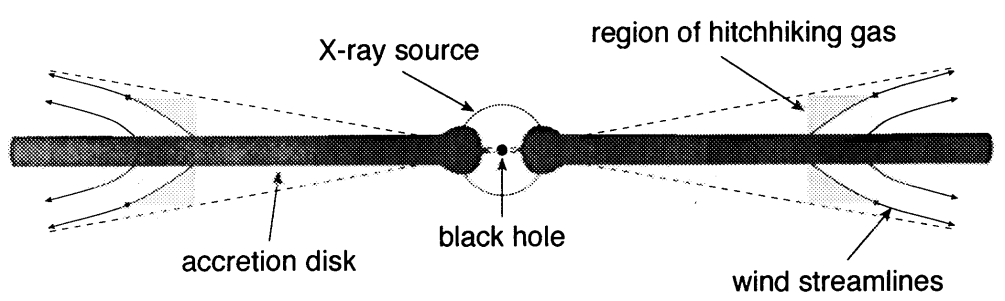
\includegraphics[width=1.0\textwidth]{figures/02-outflows/MCGV95.png}
\caption
{
{\sl Credit: Murray et al. 1995}. 
Cartoon showing the geometry of the MCGV95 model.
} 
\label{fig:MCGV95}
\end{figure}

In the MCGC95 model, a smooth wind rises from an accretion disc with a launch
radius of around $10^{16}$~cm. The wind is equatorial, with an opening angle
of $5^\circ$, and is accelerated by line forces up to a terminal velocity of $0.1c$.
A diagram of the geometry is shown in figure~\ref{fig:MCGV95}.
One of the key features of the models is the presence of a `shield' of hitchhiking
gas, which protects the outflow from X-ray over-ionization 
and allows radiation pressure on UV resonance lines to efficiently 
accelerate the flow. 

MCGV95 found that BAL profiles were
seen for an observer looking into the wind cone, and significant
line {\em emission} emerged at low inclinations. This line emission came
from a relatively small BLR ($r_{BLR} \sim10^{16}$~cm) at the base of the wind, 
where densities were high ($n_e \approx 10^{10}$~cm$^{-3}$). 
The MCGV95 model was one of the first successful disc-wind unification models,
and is especially impressive as it includes photoionization calculations and 
quantitative estimates of the resultant line EWs. However, the effects of multiple
scattering and complex radiative transfer effects could not be included 
in their calculations (see Chapter 5).

\subsection{De Kool \& Begelman: A Radiatively Driven, Magnetically Confined Wind}

It is of course possible that radiation and magnetic fields are both important
in determining the outflow characteristics. In the \cite{dekool1995} model, radiation
pressure drives an outflow from an accretion disc, and also compresses the magnetic
field lines that are dragged along with the flow. This causes the magnetic field
strength in certain regions to be comparable to the gas pressure, meaning that clouds
can be magnetically confined in the flow. A diagram is shown in figure~\ref{fig:dekool}.
The authors find that such a model would naturally emerge at a fairly equatorial
angle with a covering factor of around $10\%$, and that lower ionization material 
would be intercepted when the system was viewed from higher inclinations, potentially
explaining some of the properties of LoBALQSOs.

\begin{figure}
\centering
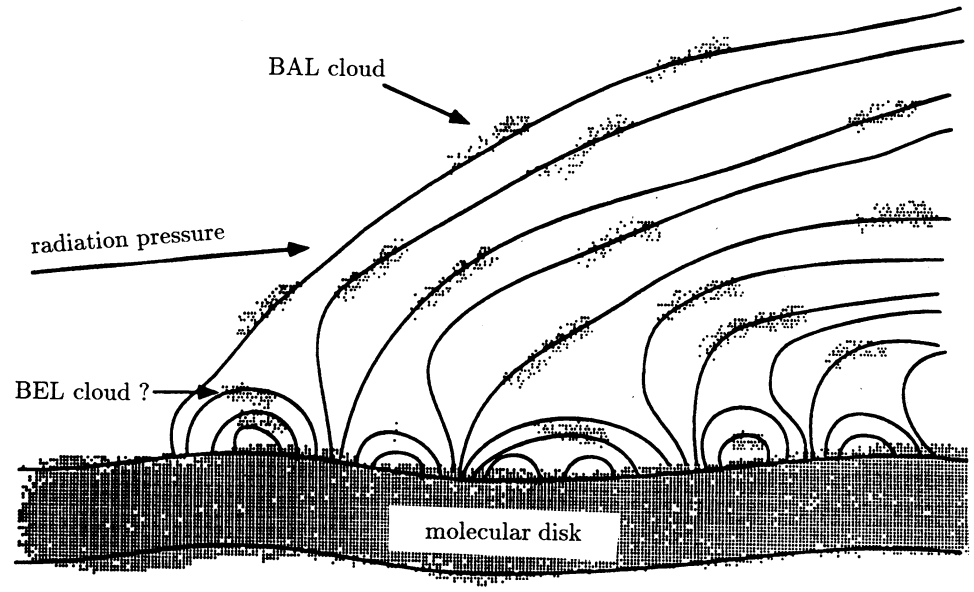
\includegraphics[width=1.0\textwidth]{figures/02-outflows/dekool.png}
\caption
{
{\sl Credit: De Kool \& Begelman 1995}. 
} 
\label{fig:dekool}
\end{figure}


\subsection{Elvis 2000: A Structure for Quasars}

\cite{elvis2000} expanded on the work of MCGV95 by proposing a simple
biconical model, empirically derived to explain as much of quasar phenomenology
as possible within one unifying framework. The geometry of the Elvis model
is shown in figure~\ref{fig:elvis}. As in the two previous models, observers 
looking into the wind cone will see a BALQSO, whereas observers looking down onto
the wind will see a type 1 quasar. Initially, the wind rises vertically, so
that observers looking underneath the flow will see NALs
due to the small range of velocities intercepted by their line of sight. 

The flow conserves angular momentum, such that the initial Keplerian velocities
determine the BEL widths, before accelerating to BAL-like velocities of $\sim0.1c$.
The wind is assumed to be two-phase, with BEL and BAL clouds embedded in 
a warm, highly ionized medium (WHIM). This WHIM is responsible for WA-like absorption
and the X-ray scattering phenomena seen in AGN. It is also responsible for confining
the BAL and BEL clouds, allowing high densities and cooler temperatures to exist
within the flow. The ionization structure for the wind is stratified, such that the material
further out along the disc plane is somewhat shielded from the inner disc and X-rays.
This allows the lower ionization BEL profiles to form in the right locations,
and also means that LoBAL profiles would be seen at a subset of inclinations.

\begin{figure}
\centering
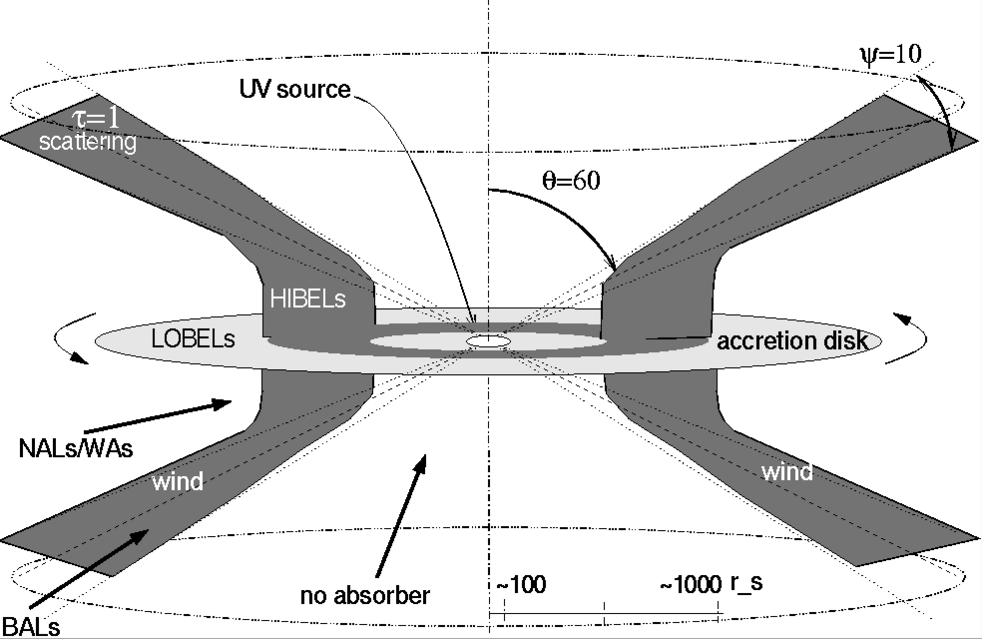
\includegraphics[width=1.0\textwidth]{figures/02-outflows/elvis.png}
\caption
{
{\sl Credit: Martin Elvis}. 
A schematic showing the main features of the Elvis model. A biconical
wind rises from an accretion disc, and the observed spectrum is determined 
purely by the viewing angle of the observer.
} 
\label{fig:elvis}
\end{figure}

\subsection{Proga et al.: Line-driven Hydrodynamic Models for AGN and CVs}



\begin{figure}
\centering
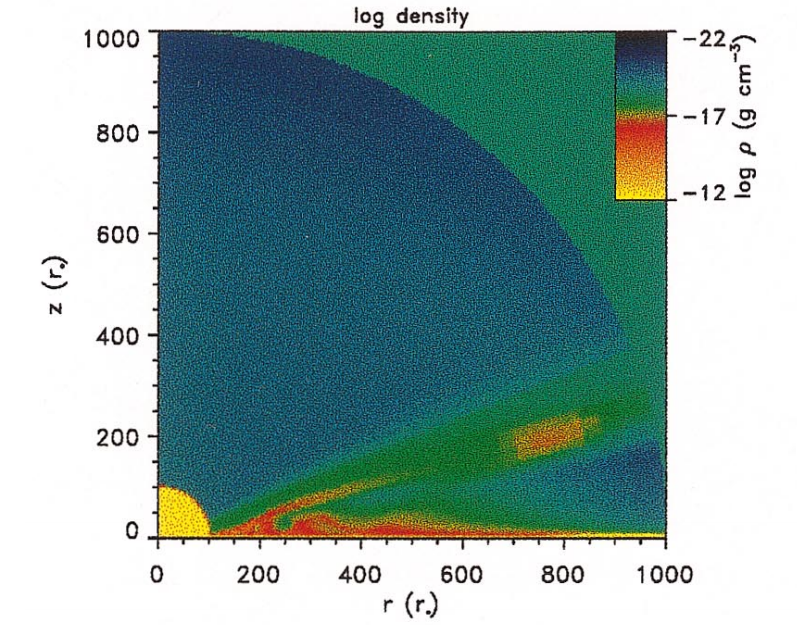
\includegraphics[width=1.0\textwidth]{figures/02-outflows/proga2.png}
\caption
{
{\sl Credit: Proga, stone \& Kallman 2000}. 
Density structure of the PSK00 model.
} 
\label{fig:PK04}
\end{figure}

Ideally, full radiative transfer and hydrodynamical simulations would be used
to estimate the viability of line-driven winds. Our team is currently working 
on this problem \citep[see][for a first step]{H14}; however, much 
can also be learned from simpler, kinematic prescriptions for outflows, which
can then be treated with full radiative transfer and ionization treatments.  

\section{A Kinematic Prescription}

\citep[][hereafter SV93]{SV93} expanded on the work of the stellar wind community
\citep[e.g.][]{AL85} 
in proposing a kinematic prescription for an accretion disc wind. Unlike 
hydrodynamical models, this model has no real predictive power in terms of velocities
and mass-loss rates. Instead, one sets these quantities in advance and examines the 
resultant properties of the flow and emergent spectra. The SV93 prescription
is the most common wind model used in the radiative transfer code \py\ (see Chapter 3),
and has been used to simulate spectra for CVs \citep[][Chapter 5]{LK02, M15}, 
AM CVn systems \citep{kusterer2014} and AGN/quasars 
\citep[][Chapter 6]{higginbottom2013, M16, yong2016}. 
A similar philosophy applied to the model of \cite{KWD95}, and which has been used
with similar applications \citep{LK02, simlong2008, sim2010}, as 
well as young-stellar objects \citep[YSOs;][]{simmacro2005}.
Kinematic prescriptions have thus been a useful tool in providing quantitative
tests of conceptual models, and assessing their ability to reproduce
the observed spectra of a variety of disc wind systems.

In the SV93 parametrization, shown in figure~\ref{fig:sv_cartoon} 
a smooth, biconical disc wind emanates from the accretion disc between 
radii $r_{min}$ and $r_{max}$. The covering fraction of the outflow is 
also controlled by the inner and outer opening angles of the wind, $\theta_{min}$ and
$\theta_{max}$, and the launch angle of the other streamlines is givenby 
\begin{equation}
\theta(r_0) = \theta_{min} + (\theta_{max} - \theta_{min}) \left(\frac{r_0 - r_{min}}{r_{max} - r_{min}} \right)^{\gamma},
\label{theta}
\end{equation}
where $r_0$ is the launch radius of the streamline.

The poloidal (non-rotational) velocity field of the wind, $v_l$, is given by
\begin{equation}
v_l=v_0+\left[v_{\infty}(r_0)-v_0\right]\frac{\left(l/R_v\right)^{\alpha}}{\left(l/R_v\right)^{\alpha}+1},
\label{v_law}
\end{equation}
where $l$ is the poloidal distance along a particular wind
streamline. The terminal velocity along a streamline, $v_{\infty}$, is
set to a fixed multiple of $v_{esc}$, the escape velocity at the launch
point. The launch velocity from the disc surface, $v_0$, is assumed to
be constant (set to $6$~km~s$^{-1}$). Once the wind is launched, it
accelerates, reaching half of its terminal velocity at $l = R_v$. The
velocity law exponent $\alpha$ controls how quickly the wind
accelerates. Larger values of $\alpha$ cause the main region of 
acceleration to occur close to $R_v$, whereas smaller values
correspond to fast acceleration close to the disc (see
Fig.~\ref{acc_law}). The rotational velocity $v_\phi$ is 
Keplerian at the base of the streamline 
and the wind conserves specific angular momentum, such that
\begin{equation}
v_\phi r = v_{k} r_0,
\label{v_law}
\end{equation}
where $v_{k}=(GM_{WD}/r_0)^{1/2}$.

\begin{figure}
\centering
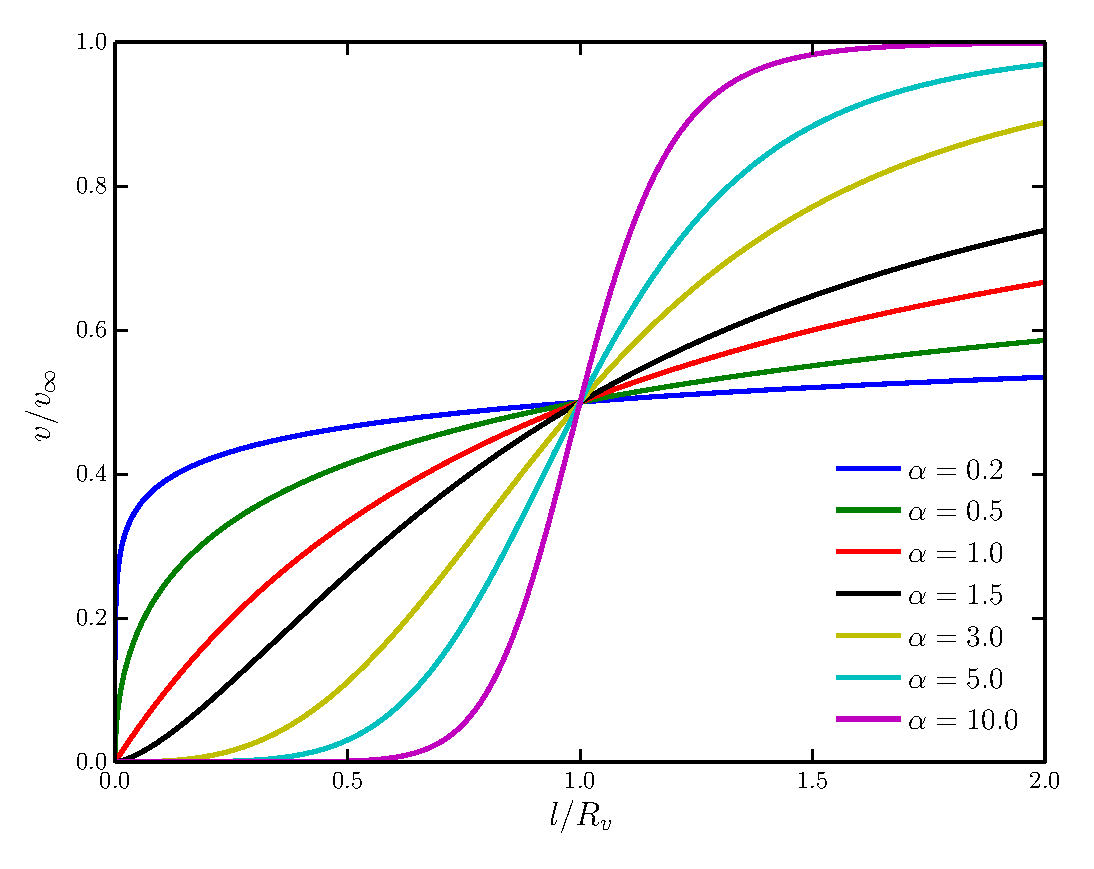
\includegraphics[width=1.0\textwidth]{figures/05-cvpaper/acc_law.eps}
\caption{
The SV93 velocity law for various values of the
acceleration exponent, $\alpha$.
%%{\bf JM: KSL has suggested we ditch this}
} 
\label{acc_law}
\end{figure}




\section{The big picture: AGN Feedback}
\label{sec:agn_feedback}

The event horizon of a $10^9~M_\odot$ BH is approximately 
$10^{15}$~cm across, a billionth of the size of a typical galactic bulge. This is 
roughly the difference in size between a small coin and the 
Earth. Even the sphere of gravitational influence of the BH is roughly 
$1000$ times smaller than the size of the galactic bulge.
Despite this vast different in scale, there is evidence
that the physics on the scale of the gravitational
radius of the BH really does affect the evolution and dynamics of its host galaxy.
When considering the {\em energetics} of accretion this becomes less surprising.
The binding energy of a galactic bulge is 
\begin{equation}
E_{bulge} \approx M_{bulge} \sigma_*^2,
\end{equation}
while the energy released in growing a black hole to a 
mass $M_{BH}^\prime$ is (assuming $\eta=0.1$)
\begin{equation}
E_{BH} \approx 0.1 M_{BH} c^2.  
\end{equation}
By combining the above two equations, and putting in typical numbers of
$\sigma_* = 0.001c$ and $M_{BH} / M_{bulge} = 10^{-3}$ we can show that 
\begin{equation}
\frac{E_{BH}}{E_{bulge}} \approx 10^{-4} \left( \frac{c}{\sigma_*} \right)^2 \sim 10.
\end{equation}
In other words, the energy released when growing a BH can exceed
the binding energy of the galactic bulge. This energetic 
argument is not alone sufficient to claim that the accreting BH must affect its
host. For example, if the radiated energy never experienced an 
optical depth of $\sim 1$ then it would clearly not couple to the galactic bulge. However,
we have already seen that many outflows in AGN possess kinetic luminosities that
are significant compared to the bolometric luminosity. Thus, outflows 
(and jets) may provide a mechanism by which the vast accretion energies can
be transferred to the BH environment.

\subsection{Observational evidence for feedback}

{
\color{blue}
Go over the various pieces of observational evidence for feedback
and the role of winds.
}
\bigskip

Perhaps the most famous pieces of evidence for some kind of long-distance 
relationship between a central BH and its host galaxy are the 
$M_{BH}-\sigma_*$ and $M_{BH}-M_{bulge}$ correlations, shown in figures~\ref{fig:msigma}
and \ref{fig:mbulge} respectively.

\nocite{mcconnell2013,gultekin2009}
\begin{figure}
\centering
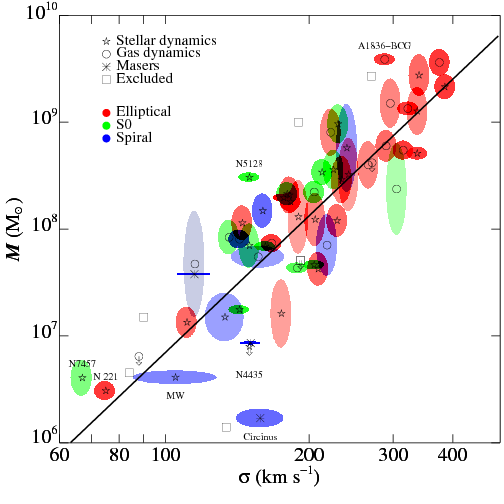
\includegraphics[width=0.7\textwidth]{figures/02-outflows/msigma.png}
\caption
{
{\sl Credit: Gultekin et al. 2009}. 
The $M_{BH}-\sigma_*$ correlation.
} 
\label{fig:mbulge}
\end{figure}

\begin{figure}
\centering
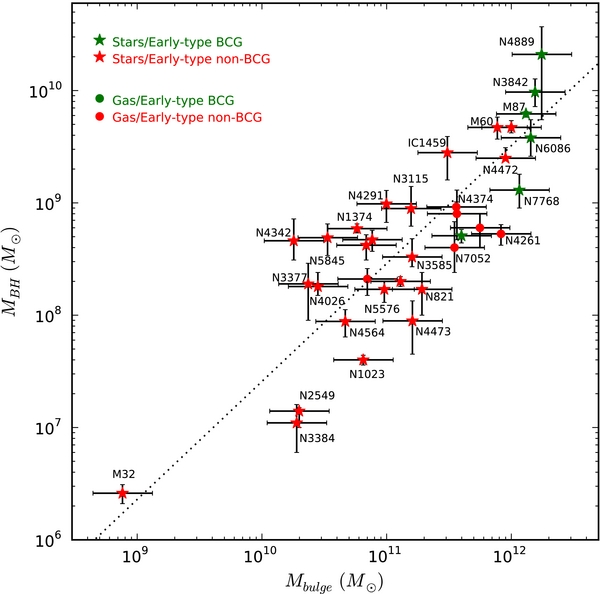
\includegraphics[width=0.7\textwidth]{figures/02-outflows/mbulge.jpg}
\caption
{
{\sl Credit: McConell \& Ma 2013}. 
The $M_{BH}-M_{bulge}$ correlation.
} 
\label{fig:mbulge}
\end{figure}

\subsection{Radiative or quasar mode feedback}

\subsection{Kinetic or radio mode feedback}

\subsection{Alternative Explanations}


